ntclass[aspectratio=169]{beamer}
\usetheme{Warsaw}
\usecolortheme{rose}
\usepackage{tikz}
\usepackage[super,square]{natbib}
\usepackage{ragged2e}
\usepackage[utf8]{inputenc}
\usepackage[english]{babel}
\usepackage[labelformat=empty]{caption}
\renewcommand{\thefootnote}{\roman{footnote}} 
%\makeatletter
\newcommand\titlegraphicii[1]{\def\inserttitlegraphicii{#1}}
\titlegraphicii{}

\setbeamertemplate{title page}
{
	\vspace{0.3in}
  \vbox{}
   %{\usebeamercolor[fg]{titlegraphic}\inserttitlegraphic\hfill\inserttitlegraphicii\par}
  \begin{centering}
    \begin{beamercolorbox}[sep=8pt,center]{title}
      \usebeamerfont{title}\inserttitle\par%
      \ifx\insertsubtitle\@empty%
      \else%
        \vskip0.25em%
        {\usebeamerfont{subtitle}\usebeamercolor[fg]{subtitle}\insertsubtitle\par}%
      \fi%     
    \end{beamercolorbox}%
    \vskip1em\par
    \begin{beamercolorbox}[sep=8pt,center]{date}
      \usebeamerfont{date}\insertdate
    \end{beamercolorbox}%\vskip0.5em
    \begin{beamercolorbox}[sep=8pt,center]{author}
      \usebeamerfont{author}\insertauthor
    \end{beamercolorbox}
    \begin{beamercolorbox}[sep=8pt,center]{institute}
      \usebeamerfont{institute}\insertinstitute
    \end{beamercolorbox}
  \end{centering}
  %\vfill
}
%\makeatother
%\author{Anirban Laha and Preksha Nema \\\vspace{0.2in} Presented By: Mitesh M. Khapra}
\author{Mitesh M. Khapra}
\title{CS7015 (Deep Learning) : Lecture 1}
\subtitle{(Partial/Brief) History of Deep Learning}
\institute{Department of Computer Science and Engineering\\ Indian Institute of Technology Madras}
\titlegraphic{
\includegraphics[height=1cm,width=2cm]{images/iitm_logo.png}}
%\titlegraphicii{\includegraphics[height=1cm,width=2cm]{logo2}}
\date{}

\newcommand\myheading[1]{%
  \par\bigskip
  {\Large\bfseries#1}\par\smallskip}

\addtobeamertemplate{navigation symbols}{}{%
    \usebeamerfont{footline}%
    \usebeamercolor[fg]{footline}%
    \hspace{1em}%
    \insertframenumber/\inserttotalframenumber
}


\begin{document}%	\author{Mitesh M. Khapra}

\title{Module 1.1}
\subtitle{Biological Neurons}
\author{}
\institute{}
\date{}

%\institute{Department of Computer Science and Engineering\\ Indian Institute of Technology Madras}
%\titlegraphic{
\includegraphics[height=1cm,width=2cm]{images/iitm_logo.png}}
%\titlegraphicii{\includegraphics[height=1cm,width=2cm]{logo2}}

\begin{frame}
	\myheading{Chapter 1: Biological Neurons}
\end{frame}

\begin{frame}
	\begin{minipage}[t][0.6\textheight][t]{\textwidth}
		\begin{columns}
			\column{0.5\textwidth}
			\begin{overlayarea}{\textwidth}{\textheight}
				\justify
				\only<1>{\myheading{Reticular Theory} Joseph von Gerlach proposed that the nervous system is a single continuous network as opposed to a network of many discrete cells!}
				\only<2>{\myheading{Staining Technique} Camillo Golgi discovered a chemical reaction that allowed him to examine nervous tissue in much greater detail than ever before\\\vspace{0.2in} He was a proponent of Reticular theory.}
				\only<3>{\myheading{Neuron Doctrine}  Santiago Ram\'on y Cajal used Golgi's technique to study the nervous system and proposed that it is actually made up of discrete individual cells formimg a network (as opposed to a single continuous network)}
				\only<4>{\myheading{The Term Neuron} The term neuron was coined by Heinrich Wilhelm Gottfried von Waldeyer-Hartz around 1891. \\\vspace{0.2in} He further consolidated the Neuron Doctrine.}
				\only<5>{\myheading{Nobel Prize} Both Golgi (reticular theory) and Cajal (neuron doctrine) were jointly awarded the 1906 Nobel Prize for Physiology or Medicine, that resulted in lasting conflicting ideas and controversies between the two scientists.}
				\only<6>{\myheading{The Final Word} In 1950s electron microscopy finally confirmed the neuron doctrine by unambiguously demonstrated that nerve cells were individual cells interconnected through synapses (a network of many individual neurons).}
			\end{overlayarea}
			\column{0.5\textwidth}
			\begin{overlayarea}{\textwidth}{\textheight}
				\begin{figure}
					\centering
					\only<1>{\includegraphics[scale=0.5]{"images/module1/1871"}}
					\only<2>{\includegraphics[scale=0.5]{"images/module1/1873"}}
					\only<3>{\includegraphics[scale=0.3]{"images/module1/1899_1"}}
					\only<4>{\includegraphics[scale=0.3]{"images/module1/1891"}}
					\only<5>{\includegraphics[scale=0.3]{"images/module1/1906"}}
					\only<6>{\includegraphics[scale=0.15]{"images/module1/1950"}}
				\end{figure}
			\end{overlayarea}
		\end{columns}
	\end{minipage}
	\begin{minipage}[t][0.4\textheight][t]{\textwidth}
		\begin{overlayarea}{\textwidth}{\textheight}
			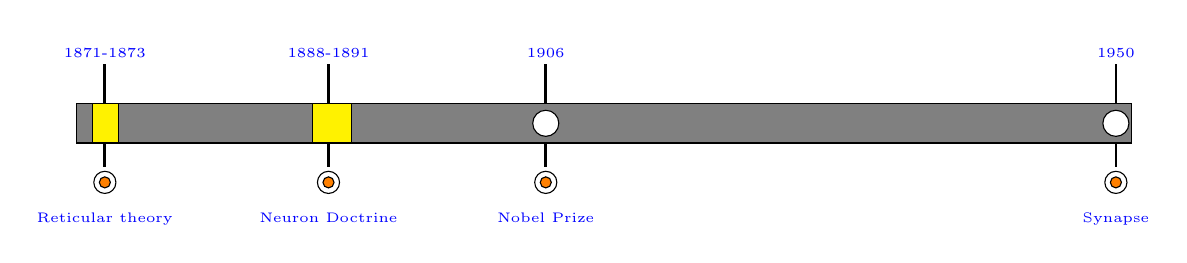
\begin{tikzpicture}[datemarker/.style={circle, draw=black,fill=white},textlabel/.style={anchor=center,text height=1.7ex,text depth=.25ex}]
				\tikzset{every node/.style={font=\tiny, color=blue}}\draw[fill=gray](-0.2,0) rectangle (13.2,0.5) node[white, below]{};

				\onslide<1->{\draw[fill=yellow] (0,0) rectangle(0.329113924051, 0.5){};}
				\onslide<1->{\draw [line width=1pt] (0.16, 0.5) to (0.16, 1.0);}
				\onslide<1->{\draw (0.16, 1.2) node [textlabel] {1871-1873 };}
				\onslide<1->{\draw [fill=orange](0.16, -0.5) circle (2pt){};}
				\onslide<1->{\draw (0.16, -0.5) circle (4pt){};}
				\onslide<1->{\draw [line width=1pt] (0.16, 0) to (0.16, -0.3);}
				\onslide<1->{\draw (0.16,-0.9) node [textlabel] {Reticular theory};}

				\onslide<3->{\draw[fill=yellow] (2.79746835443, 0) rectangle(3.29113924051, 0.5){};}
				\onslide<3->{\draw [line width=1pt] (3, 0.5) to (3, 1.0);}
				\onslide<3->{\draw (3, 1.2) node [textlabel] {1888-1891 };}
				\onslide<3->{\draw [fill=orange](3, -0.5) circle (2pt){};}
				\onslide<3->{\draw (3, -0.5) circle (4pt){};}
				\onslide<3->{\draw [line width=1pt] (3, 0) to (3, -0.3);}
				\onslide<3->{\draw (3,-0.9) node [textlabel] {Neuron Doctrine};}

				\onslide<5->{\node at (5.75949367089, 0.25) [datemarker] {};}
				\onslide<5->{\draw [line width=1pt] (5.75949367089, 0.5) to (5.75949367089, 1.0);}
				\onslide<5->{\draw (5.75949367089, 1.2) node [textlabel] {1906 };}
				\onslide<5->{\draw [fill=orange](5.75949367089, -0.5) circle (2pt){};}
				\onslide<5->{\draw (5.75949367089, -0.5) circle (4pt){};}
				\onslide<5->{\draw [line width=1pt] (5.75949367089, 0) to (5.75949367089, -0.3);}
				\onslide<5->{\draw (5.75949367089,-0.9) node [textlabel] {Nobel Prize};}

				\onslide<6->{\node at (13.0, 0.25) [datemarker] {};}
				\onslide<6->{\draw [line width=1pt] (13.0, 0.5) to (13.0, 1.0);}
				\onslide<6->{\draw (13.0, 1.2) node [textlabel] {1950 };}
				\onslide<6->{\draw [fill=orange](13.0, -0.5) circle (2pt){};}
				\onslide<6->{\draw (13.0, -0.5) circle (4pt){};}
				\onslide<6->{\draw [line width=1pt] (13.0, 0) to (13.0, -0.3);}
				\onslide<6->{\draw (13.0,-0.9) node [textlabel] {Synapse};}
			\end{tikzpicture}
		\end{overlayarea}
	\end{minipage}
\end{frame}
\end{document}
